\chapter{Background}
% "Ongelmakentän esittely".

On this chapter the three prime themes around this thesis are introduced. Basic knowledge of these themes are required in order to fully comprehend all the aspects on the case study investigated on this thesis later on. 

The basics of \textit{single-page application} paradigm is introduced as it is the method how the web application is built on the case study. The concept of \textit{computer supported collaborative work} is introduced since the case study's application is essentially that: multiple users collaboratively viewing and editing the same data set. The most usual types of \textit{Internet connectivity issues} and the reasons for them are portrayed, since the disruption created by them to the case study's application created the actual need for offline supported functionalities in the first place. 




%% ----------------------------------
\section{Single-Page Applications}
% TODO: % näitä kerätty tänne sitä mukaa kun kirjoitettu implementationia
% - rise of the javascript, (1995 ja netscape?), siitä jotain?=


% - yleisesti tuotantojavaskriptistä, yks yhdistetty&minimifoitu .js-möykky tuotannossa (tähän viittaan implementaatio-osuudessa)?
% - AMD-moduulin avaus?


In the past decade the software industry as a whole has been facing a major paradigm shift on the way how and where applications are developed and operated. Progress in web technologies and standards have made possible for the browser environment to be a more and more powerful but still universal computing platform. Software applications that were previously build for different kind of operating system and CPU combinations are now written with web technologies and ran on the browser. This change is mainly accomplished by the power of distribution the web platform provides. Software provider or the organization's IT function doesn't have to take care of updating end user software to the latest version anymore, because the client-server paradigm [Berson] makes running outdated software version virtually impossible. In a traditional desktop application patching the software to fix bugs or introducing a new feature requires downloading a installer or a patcher and then it must be ran on the computer. This requires action from the user or from the IT function. This might not cover the whole upgrading process in every situation: sometimes updating dependent libraries or operating system might be required. It also enables possibility for different computers to be running different versions of the software, creating circumstances for version mismatches between different clients. [jazayeri 3.3] [taivalsaari_mashware:_2009]

The move from individual installations to a centralized reverses the general model how software is operated since the start of the personal computing revolution [jazayeri 3.3]. As stated above, this comes with many benefits. One of the most important ones is the (almost) unified platform provided for the developers. Thanks to automatic update mechanisms of the modern browsers, this platform is one of the fastest updating ones there is when it comes to speed of patches applied to end user computers [duebendorfer and frei]. Due to the easiness of the deployment process, it is not unusual to see web application rolling in releases to production on daily or even on hourly basis [jazayeri 3.3].

Executing complicate applications on the web platform has been made possible by the evolution of the web pages from "classic", static presentation consisting of single pages to an interactive and collaborative web applications. On the early phases of World Wide Web user navigated through hyperlinks within single pages each of them being formed and served by the server. Client, the browser, was responsible only for rendering the response of the server. [taivalsaari_mashware:_2009] The current state of technology allows more of the functionality to be moved or duplicated from the server to the client. When before web pages on the browser were stateless, and the state transforms were done while moving to a new page, now it is possible for the browser to handle the state transitions and retrieve only the needed data from the server when required via AJAX-requests. [building rich web applications with ajax] 

The application state handling on the browser environment and the increased amount of possibilities on the browser creates the basis for modern web development and the platform for the offline feature: the single-page application. Single-page application is tightly relevant to other hype terms such as Web 2.0 and the nowadays partly old-fashioned term DHTML. All single-page applications could be called Web 2.0 applications, but not all Web 2.0 applications are single-page applications. Whereas traditional web pages where synchronously fetched and generated by the web server, single-page application relies on asynchronous pattern on data fetching. [garrett] With the asynchronous pattern the browser can fetch resources on smaller chunks when the need arises, usually through REST APIs [masse]. This also makes possible the premise for an \textit{occasionally connected application}, meaning that the web application can function without having a continous Internet connection [Casario et al]. This widens a lot the range of use cases which can be covered by web applications.



% ###
\subsection{REST API}
% - JSON -termin avaus?
% - REST API:sta jotain (Päikky cachettaa nimenomaan tämäntyyppisiä requesteja)\citation{taivalsaari_mashware:_2009}
% - kuva havainnollistamaan että SPA hakee resursseja yksitellen ja vanhassa mallissa haetaan kokonaisia sivuja?
% - tarviikohan AJAXista tänne jotain?






% ###
%\subsection{MVC Architecture}
% - MVT -termin avaus?
% ---> ennen vain view selaimessa, backbonessa koko härveli
% ---> "Frontend gets fatter and fatter" -> Päikyn tilakone myös frontendissä nyt, bisneslogiikka duplikoitava/siirrettävä clienttiin
% - jQuery?







%% ----------------------------------
\section{Computer Supported Collaborative Work}
"Reaaliaikaisesta informaationjaosta päiväkotiympäristössä"
- verkkovälitteinen vuorovaikutus
- hakusanalla computer supported collaborative work (CSCW) löytyy kamaa 
- web 2.0 on nimeomaa tätä??



%% ----------------------------------
\section{Internet Connectivity Issues}
% vai pelkkä "Internet Connectivity"?
% http://dl.acm.org/citation.cfm?id=2307649 ?
 - eri tavat yhdistää internetiin (piuhayhteys, wlan, mobiilidata)
 - kännyverkon toiminnasta jotain?

 - kännyverkon toimivuuden vaihtelun yleisyydestä
 - yleisimmät ongelmatilannetyypit

% Minkälaisia offline ratkaisuja on olemassa web/känny-puolella (miten google/microsoft yms. ovat lähestyneet ongelmaa)?
% % onko muita kenttäkokeita tehty offline-moodiin liittyen??



%% ----------------------------------
\section{Research Gap}
% -> Gappiin ehkä jotain, että verkkovälitteistä vuorovaikutusta on tutkittu paljon (katso CSCW kamaa) ja että mobiiliverkojen tutkimus/kehitys/käyttö ollut räjähdymäistä. Kuitenkaan ei ole paljoa tutkimusta siitä kuinka verkon katkeaminen vaikuttaa reaalisaikaista tiedonvälitystä vaativan sovelluksen käyttökokemukseen ja kuinka sovellussuunnittelussa tulisi katkot ottaa huomioon. 


% This chapter focuses on the background of today's web applications and the literature that relates to the circumstances causing the connectivity issues. This chapter addresses the basics of today's web technologies and the methods that makes offline supported features possible. This chapter coverages also briefly principles on mobile device communication on the network layer, the ideology on Computer Supported Collaborative Work and takes a glimpse on already existing efforts done on solving the offline issue in web applications.  % VANHA INTRO-intro


% "Tämän dipan käsittelemä aihe sijaitsee kolmen edellisen kappaleen keskiössä -> CSCW mahdollistettuna SPA:na mutta Internet-yhteyden katkeamisten riivaamana -> whattodo"

\begin{figure}[t]
\begin{center}
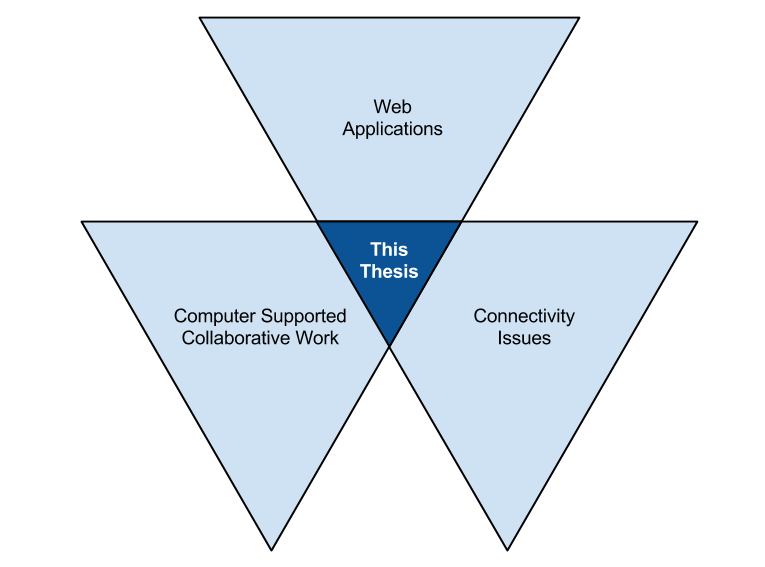
\includegraphics[width=0.8\textwidth]{assets/researchgap.png}
\end{center}
\caption{The research gap covered by this thesis}
\label{fig:researchgap}
\end{figure}










% toistaiseksi hyllytetty kappale, nämä asiat tohon internet connectivity issuesiin messiin
%% ----------------------------------
% \section{Existing Solutions for the Offline Problem}
